%### 
\subsection{System Components}
%### 
\label{sec:components}
Extending \xmlmate to support binary subjects has greatly benefited from frameworks described in
\cref{sec:tech} as they help solve the majority of the arising subtasks rather easily. The following
paragraphs describe the components involved in the new extended \xmlmate work process.
%###  
\paragraph{XMLMate Core} ~\\
%### 
  The \java application \xmlmate performs its genetic operations on a population of chromosomes; this 
  results in a set of \xml files, whose fitness needs to be determined according to the currently employed
  fitness function. The paths to these files are then sent out via a \zmq socket either directly to the
  \emph{test drivers}, in case the program being tested supports reading inputs in \xml format, or alternatively 
  to an arbitrary number of \emph{converters}, that, as the name suggests, convert the \xml files into a format 
  suitable for the system under test. This distinction is completely transparent to \xmlmate and thus allows for 
  adding an arbitrary number of transformation steps between itself and the test drivers.
  %### 
  \paragraph{Load Balancer} ~\\
  %### 
  A load balancer is responsible for managing a set of homogeneous worker nodes like converters or test
  drivers by distributing the arriving workloads fairly among them. The fair queueing provides a significant
  performance upgrade from the previously employed round robin method. Not all workloads require equal
  processing time, and because it is indeterminable a priori, the round robin workload distribution strategy
  has often caused faster work items to get ``stuck'' in queue behind slower ones, while there were idle
  workers available. The new load balancing mechanism allows to track the worker's availability and assign
  newly arriving workloads to idle workers in the least recently used order. To provide an analogy, the load
  balancer's queueing strategy has been upgraded from a supermarket to a post office. 
  
  A load balancer provides a facade for the workers it manages, so that other system components only ever
  directly interact with the balancer, but never with the workers themselves, as they are sometimes unreliable
  and can fail at any moment. The most common system setup consists of two load balancers -- one for the format
  converters and one for test drivers, so even though it says above that \xmlmate sends its work packets to
  converters or test drivers, in actuality it communicates with their respective load balancers. 
  %### 
  \paragraph{Format Converter} ~\\
  %### 
  A format converter (most of which are currently implemented in \python) receives a conversion task from
  its load balancer through a \zmq socket, which it completes by converting the file found at the location
  specified in the task message. It then responds with another message containing the location of the converted
  file. There can be an unlimited number of converters active at the same time processing multiple
  conversion requests in parallel. 
  
  The design decision to enable the converters to drop in and out at
  runtime has two very useful properties: firstly, it allows to circumvent the parallelism limitation
  imposed by Python's GIL (global interpreter lock) by being able to run multiple interpreter
  instances in parallel without them interfering; and, secondly, it makes it possible to apply meta-heuristics
  to the process by varying the number of converters dynamically depending on the load, which makes for an
  interesting future work item.
  %### 
  \paragraph{Test Driver} ~\\
  %### 
  A test driver receives a message from its balancer, which, in turn, receives it either directly from
  \xmlmate in case of an \xml based file format, or otherwise from the previous balancer (usually a
  converter's balancer), unpacks the file path, and feeds it to the system under test, which is being monitored
  by a \emph{pintool} that implements the ``client side" of the aforementioned currently employed fitness
  function. The test driver's responsibilities also include signaling the beginning and end of the execution of
  the program under test to the pintool by calling special marker methods \texttt{PIN\_SCORE\_START}
  and \texttt{PIN\_SCORE\_END}, which the pintool replaces with its own internal fitness data related
  processing methods. The driver is implemented in C and, as is the case with converters, there can
  be arbitrarily many active at the same time.
  %### 
  \paragraph{Pintool} ~\\
  %### 
  As previously mentioned, the pintool monitors the execution of the program under test and records
  data relevant to the computation of the fitness score according to the fitness function it is part of.
  E.g.\ for a fitness function that counts the number of basic blocks executed in the program, the pintool 
  would keep a set of basic blocks that it has observed being executed. The pintool replaces the call to 
  \texttt{PIN\_SCORE\_START} in the driver with a method that resets its fitness related data stores. In the 
  above example this would clear the set of executed basic blocks. The pintool also replaces the call to
  \texttt{PIN\_SCORE\_END} with a method that sends the stored data back to the balancer. 
  The pintools are implemented in \cpp and there is always exactly one pintool per test driver.
  Because each pintool runs in the same process as its test driver, it is possible to share the same \zmq
  socket between driver and pintool to communicate with the load balancer, which makes it relatively
  easy to implement the next system component.
  %### 
  \paragraph{Lifeguard} ~\\
  %### 
  A lifeguard protects the joint process of test driver, system under test and pintool from fatal application
  crashes. Whenever \xmlmate produces an input file which crashes the program under test, the entire process
  dies off without a possibility to report this valuable finding. To prevent this, a lifeguard launches a
  driver process and gives it an \emph{identity} (which is a \zmq concept -- the load balancer distinguishes
  the workers by their identities). As soon as control returns to the lifeguard, which means that the launched
  process has died, it assumes the identity of the recently deceased and reports the fact of death to the load balancer, which will transparently forward this to \xmlmate in order for the corresponding input to be
  stored. Afterwards, the lifeguard casts off the identity and relaunches the driver with it once again.
  Each test driver is being guarded by its own personal lifeguard implemented in \python.
  %### 
  \paragraph{Fitness Function} ~\\
  %### 
  The fitness function in \xmlmate receives the message from the pintool and interprets it according to 
  its specification. E.g.\ again, if the fitness function is supposed to count the number of executed basic
  blocks, it would expect to receive a set of basic block addresses. Finally, the  fitness function assigns the
  computed fitness score to the genetic representation of the \xml file sent out in step 1, unless the message
  says that the corresponding input has caused a test driver to die, in which case the genetic representation
  will receive the worst fitness score to be removed from the population in order not to continuously keep
  crashing the test drivers, and the input file itself will be kept permanently.

%### 
\paragraph{Overview} ~\\
%### 
\Cref{fig:components} provides a schematic overview of the aforementioned components and which other components 
they interact with inside the system. The visualization also shows that the system scales out to \texttt{n}
format converters and \texttt{m} \emph{workers} --
a collective noun summarizing a test driver, its pintool, the program under test, and their lifeguard
instance.

\begin{figure}[htb]
\centering
  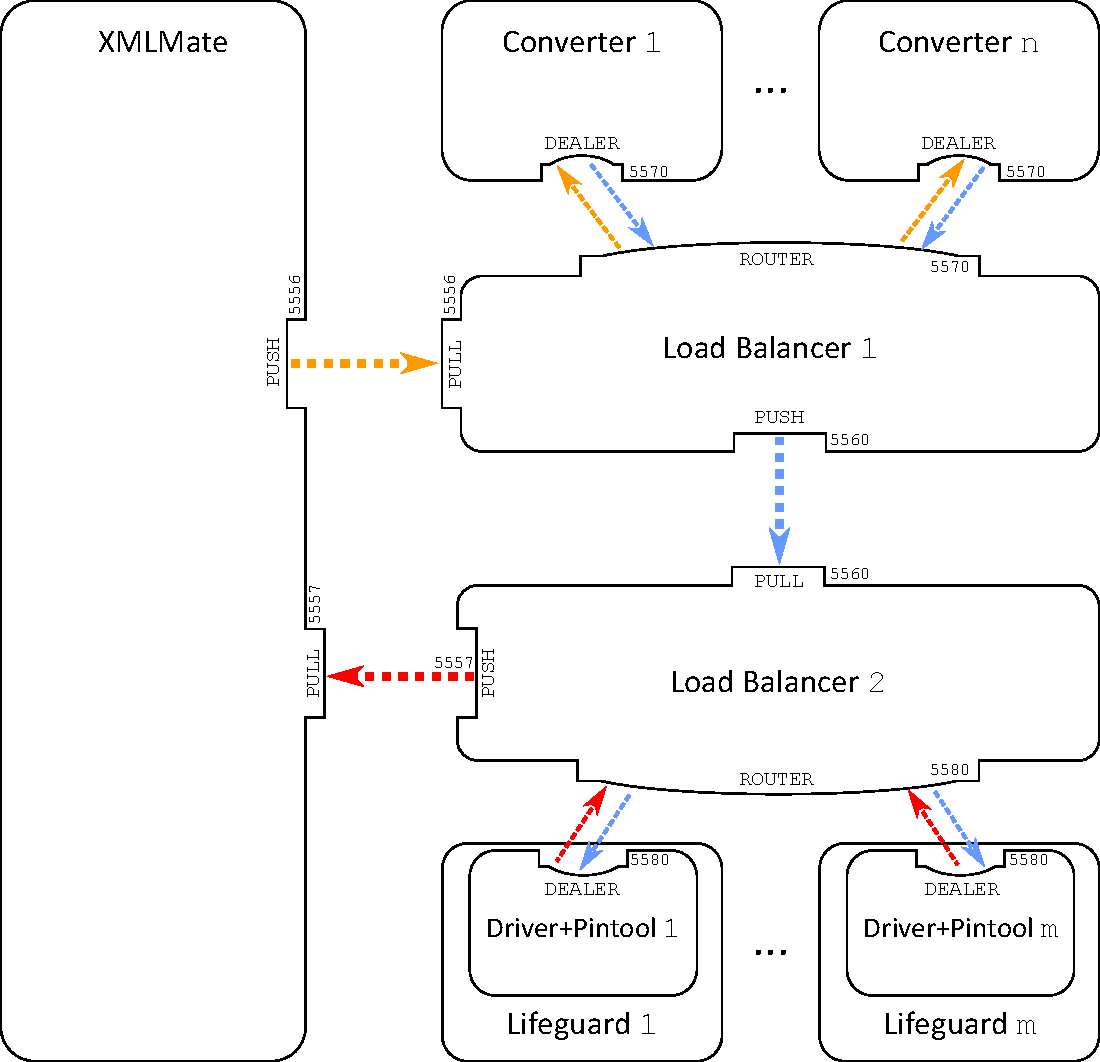
\includegraphics[width=\columnwidth]{system.pdf} 
  \caption{The Components of \xmlmate. 
  The arrows demonstrate the flow of data between the system components. Orange arrows denote the work items
  in \xml format sent out by \xmlmate itself, the blue arrows show the flow of converted files, and the red
  arrows signify the way the fitness information takes.
}
  \label{fig:components}
\end{figure}

%### 
\paragraph{Development Mockups} ~\\
%### 
When developing such a diverse ecosystem it is important to be able to inspect and test each component
individually, so as not to lose track of any important details, and to be able to isolate faults efficiently
without having to keep the entire system in the focus of attention. 
This is best accomplished by constructing
very lightweight mockup versions of the most important system components, so that the entire system does not
have to be launched when concentrating on a single component. Instead, only the single real component under
investigation has to be started, while the rest of the system is being simulated by the ``bare bones''
component mockups.

Examples for such mockup components that were used during development include two test driver mockups -- one
written in \java and one in C, which were used to test basic \zmq connectivity and
cross-language \msgpack serialization/deserialization respectively. Several mockups for the system under test
were used to test the \java parts of \xmlmate's fitness functions by simply sending random data in the
required \msgpack format without requiring any binary instrumentation. There is also a mock version of
\xmlmate itself, which sends out work items that consist of hardcoded file paths, alleviating the need to
constantly generate new input files, as well as providing deterministic inputs as a means to test the
consistency of values reported by the pintool components of fitness functions. Having this mockup send out
predefined work items also allows to skip the format conversion phase, which further lightens the complexity
of the system.

In most cases, when implementing new components of a system from scratch, I found it to be very advisable to
start with their mockup version, as the effort is usually worthwhile since any mistakes can be caught
cheaply and early on and most of the code is directly transferable to the finished component.
\FloatBarrier